\chapter{质点动力学（上）}
\setcounter{example_counter}{1}
\section{牛顿运动定律}

%\subsection{牛顿运动定律的内容}

\begin{itemize}
    \item 牛顿第一定律：任何物体都保持静止或匀速直线运动的状态，除非作用在它上面的力迫使它改变这种状态
    \item 牛顿第二定律：运动的变化与所加的动力成正比，并且发生在这个力所沿的直线方向
    \begin{formula}
        $\vec{F}=\dfrac{d\vec{p}}{dt}=m\dfrac{d\vec{v}}{dt}=m\vec{a}$
    \end{formula}
    \item 牛顿第三定律：两个物体对各自对方的相互作用总是相等的，而且指向相反方向
\end{itemize}

\warn{注意，牛顿运动定律仅在惯性参考系中成立，且仅适用于宏观物体的低速运动。}

%\subsection{牛顿第二定律的应用}

\begin{example}{牛顿第二定律与微积分结合}
    汽艇关掉发动机后，因水面阻力而逐渐减速。设关机后速度为$v_0$，阻力大小为$kv$，汽艇质量为$m$，求$t$时刻的速率和停止前通过的路程。

    \tcblower

    (1)~根据牛顿第二定律，$F=-kv=m\dfrac{dv}{dt}$，分离变量得$\dfrac{dv}{v}=-\dfrac{k}{m}dt$

    \vspace{0.5em}

    两边分别积分$\displaystyle\int{\dfrac{dv}{v}}=-\int{\dfrac{k}{m}dt}$，得$\ln{v}=C-\dfrac{k}{m}t$
    
    \vspace{0.25em}

    初始条件为$t=0$时，$v=v_0$，代入求得$C=\ln{v_0}$. 代回整理得$v=v_0 e^{-\frac{k}{m}t}$

    \vspace{0.25em}

    (2)~位移$x=\displaystyle \int_0^t{v_0 e^{-\frac{k}{m}t}dt}=\dfrac{m}{k}v_0(1-e^{-\frac{k}{m}t})$，
    当$t\rightarrow \infty$时，$x\rightarrow \dfrac{m}{k}v_0$，这就是停止前通过的路程。
   
    \tcbline
    
    \noindent
    【补充练习】质量为$m$的物体由静止下落，空气阻力大小为$kv$，求任意时刻的速度和收尾速度。
\end{example}

\section{机械能守恒}

\subsection{功与功率}

\subsubsection{功}

力对物体做的功，定义为力与作用点位移的数量积。特别地，恒力做功$W=\vec{F}\cdot \Delta \vec{r}$
\begin{formula}
    $dW=\vec{F}\cdot d\vec{r},~~W=\displaystyle\int{\vec{F}\cdot d\vec{r}}$
\end{formula}

\note{一些教材将功的符号写成$A$，这种写法源于德语，但国家标准规定为$W$.}

\subsubsection{功率}

单位时间内的功称为功率。平均功率等于做功除以时间，瞬时功率等于力与速度的数量积。
\begin{formula}
    $\bar{P}=\dfrac{W}{t},~P=\vec{F}\cdot \vec{v}$
\end{formula}

\begin{example}{做功的计算}  
    质点在几个力的作用下在平面上运动，运动方程$\vec{r}=t\hat{i}+t^2\hat{j}$. 求下面几个力在$t=\SI{1}{s}$和$t=\SI{2}{s}$之间所做的功。并求出第(1)个力在这段时间内的平均功率、$t=\SI{2}{s}$时的瞬时功率。

    (1)~$\vec{F}=5\hat{i}+5\hat{j}$,~(2)~$\vec{F}=5x\hat{i}+5y\hat{j}$,~(3)~$\vec{F}=5y\hat{i}+5x\hat{j}$

    \tcblower

    (1)~这个力是恒力，只需求出位移。
    
    在$t=\SI{1}{s}$和$t=\SI{2}{s}$时刻，位矢$\vec{r}_1=\hat{i}+\hat{j},~\vec{r}_2=2\hat{i}+4\hat{j}$，位移$\Delta \vec{r}=\hat{i}+3\hat{j}$

    \vspace{0.5em}

    所以做功$W=\vec{F}\cdot \Delta \vec{r}=(5,5)\cdot (1,3)=\SI{20}{J}$，平均功率$\bar{P}=\dfrac{W}{t}=\SI{20}{W}$

    \vspace{0.5em}

    要求瞬时功率，需要先求出速度。用运动方程求导可得$\vec{v}=\dfrac{d\vec{r}}{dt}=\hat{i}+2t\hat{j}$

    \vspace{0.2em}

    所以$t=\SI{2}{s}$时速度为$\vec{v}=\hat{i}+4\hat{j}$，瞬时功率$P=\vec{F}\cdot \vec{v}=(5,5)\cdot (1,4)=\SI{25}{W}$

    (2)~上一问已求出质点位置从$(1,1)$运动到$(2,4)$，所以$x,y$的变化范围分别是$1\rightarrow 2$和$2\rightarrow 4$。

    \vspace{0.3em}

    做功$W=\displaystyle\int_1^2{F_xdx}+\displaystyle\int_1^4{F_ydy}=\displaystyle\int_1^2{5xdx}+\displaystyle\int_1^4{5ydy}=\SI{45}{J}$

    \vspace{0.3em}

    (3)~根据$x=t,y=t^2$，可求出轨迹方程$y=x^2$，也可得到$x=\sqrt{y}$

    \vspace{0.3em}
    
    做功$W=\displaystyle\int_1^2{F_xdx}+\displaystyle\int_1^4{F_ydy}=\displaystyle\int_1^2{5ydx}+\displaystyle\int_1^4{5xdx}=\int_1^2{5x^2dx}+\displaystyle\int_1^4{5\sqrt{y}dy}=\SI{35}{J}$

    \tcbline

    【补充练习】质点在几个力的作用下从原点运动到$\vec{r}=2\hat{i}-3\hat{j}$的位置，其中一个力是$\vec{F}_1=-5\hat{i}+2\hat{j}$，还有一个力是$\vec{F}=2x\hat{i}-4y\hat{j}$，求这两个力所做的功。
\end{example}

\subsection{动能定理}

对于质点而言，合力对质点做的功，等于质点的动能变化。

对于质点系而言，所有内力和外力做的总功，等于质点系动能的变化。

%\warn{质点系的动能定理要考虑内力做功。}

\begin{formula}
    质点：$W=\Delta E_k$；质点系：$W_{\text{内}}+W_{\text{外}}=\Delta E_k$
\end{formula}

\begin{example}{动能定理}
    质量为$m=\SI{2}{kg}$的质点沿$x$轴正方向运动，合外力$F=8+8x$（SI），若物体从原点出发，初速度为$\SI{2}{m/s}$，求：(1)~运动到位置$x$时的速度；(2)~$x$与$t$的关系。
    \tcblower

    (1)~在从原点运动到位置$x$的过程中，做功$W=\displaystyle\int_0^x{(8+8x^2)dx}=8x+4x^2$

    \vspace{0.5em}

    根据动能定理，$W=8x+4x^2=\dfrac{1}{2}mv^2-\dfrac{1}{2}mv_0^2$，代入$v_0=2$，得$v=2(x+1)$

    \vspace{0.5em}

    (2)~根据上一问结果，$v=\dfrac{dx}{dt}=2(x+1)$，分离变量得$\dfrac{dx}{x+1}=2dt$

    \vspace{0.5em}

    两边同时积分$\displaystyle\int{\dfrac{dx}{x+1}}=\int{2dt}$，得$\ln{(x+1)}=2t+C$

    \vspace{0.25em}

    初始条件为$t=0$时，$x=0$，代入求得$C=0$.~整理得$x=e^{2t}-1$

    \tcbline

    【补充练习】质量为$m=\SI{2}{kg}$的质点沿$x$轴运动，合外力$F=10+6x^2$，若物体从原点静止出发，求运动到$x=\SI{4}{m}$时的速度大小。
    
\end{example}

\subsection{保守力与势能}

\subsubsection{保守力}

做功与路径无关的力称为\textbf{保守力}。沿任意路径转一圈，保守力的做功为零。

\note{重力、万有引力、弹簧弹力是保守力；摩擦力、爆炸力不是保守力，非保守力不能定义势能。}

\subsubsection{势能}

保守力可定义势能$E_p$，保守内力做功等于势能的减少量。

\begin{formula}
    $W_{\text{保}}=-\Delta E_p=E_{p\text{初}}-E_{p\text{末}}$
\end{formula}

\note{势能的数值与势能零点的选择有关，但有意义的只有势能的变化量。}

\subsubsection{常见保守力的势能}

\begin{table}[htb]
    \centering
    \begin{tabular}{|c|c|c|c|}
        \hline
        保守力 & 表达式 & 默认势能零点 & 势能 \\
        \hline
        重力 & $F=-mg$ & 地面 & $E_p=mgh$ \\
        \hline
        \rule{0pt}{18pt}\rule[-12pt]{0pt}{0pt} 万有引力 & $F=\dfrac{GMm}{r^2}$ & 无穷远处 & $E_p=-\dfrac{GMm}{r}$ \\
        \hline
        \rule{0pt}{18pt}\rule[-12pt]{0pt}{0pt} 弹簧弹力 & $F=-kx$ & 原长 & $E_p=\dfrac{1}{2}kx^2$ \\
        \hline
    \end{tabular}
\end{table}

\begin{example}{保守力做功}
    设地球质量为$M$，半径为$R$。(1)~推导万有引力势能的表达式；(2)~若质量为$m$的飞船仅在万有引力的作用下，从距地心$r_1$处下落到$r_2$处，求飞船动能增量；(3)~若地球从地面发射一个飞船，速度多大时能脱离地球？（即第二宇宙速度）
    
    \tcblower

    (1)~从无穷远处到距离为$r$处，万有引力做功$W=\displaystyle\int_\infty^r{-\dfrac{GMm}{x^2}dx}=\left.\dfrac{GMm}{x}\right|_\infty^r=\dfrac{GMm}{r}$

    \vspace{0.35em}

    万有引力势能等于万有引力做功的相反数，$E_p=-\dfrac{GMm}{r}$

    \vspace{0.35em}
    
    (2)~$\Delta E_k=W_{\text{保}}=E_{p\text{初}}-E_{p\text{末}}=-\Delta E_p=\left(-\dfrac{GMm}{r_1}\right)-\left(-\dfrac{GMm}{r_2}\right)=GMm\left(\dfrac{1}{r_2}-\dfrac{1}{r_1}\right)$

    \vspace{0.35em}

    (3)~要想脱离地球，则需要能运动到无穷远处。因为$E_k\geq 0$，所以满足条件的最小速度应使$E_k=0$.

    \vspace{0.35em}
    
    由能量守恒，$\dfrac{1}{2}mv^2+\left(-\dfrac{GMm}{R}\right)=E_k$，令$E_k=0$，解得$v=\sqrt{\dfrac{2GM}{R}}$。
    
    \tcbline
    【补充练习】判断下列说法是否正确：
    
    (1) 若保守力做正功，则相应的势能增加；(2) 若质点经过一闭合路径运动一周，则保守力做功为零；
    
    (3) 作用力与反作用力的做功之和一定为零；(4) 质点系动能的变化等于外力所做的功。
    
\end{example}

\subsection{功能原理与机械能守恒定律}

\subsubsection{功能原理}

质点系所受外力和非保守内力做的功，等于系统机械能的变化量。

\begin{formula}
    $W_{\text{内非}}+W_{\text{外}}=\Delta E$
\end{formula}

\subsubsection{机械能守恒定律}

若只有保守内力做功，则质点系的机械能守恒。

\begin{example}{功能原理与机械能守恒}
    均匀链条总长为$L$，质量为$M$，放在桌面上并使一部分下垂，下垂的长度为$a$. 链条由静止开始运动，直至刚好离开桌面。(1)~若桌面光滑，求刚离开桌面时的速率；(2)~若滑动摩擦因数为$\mu$，求刚离开桌面时的速率。
    
    \tcbline
    \begin{minipage}{0.75\textwidth}
    \setlength{\parskip}{0.5em}
    \linespread{1.3}

    (1)~对比初末状态，只有桌面上$L-a$长度的链条发生变化

    \vspace{0.2em}
    
    这一段链条的质量为$\dfrac{L-a}{L}M$，重心位置下降了$a+\dfrac{L-a}{2}=\dfrac{L+a}{2}$
    \end{minipage}
    \hfill
    \begin{minipage}{0.22\textwidth}
        \vspace{-0.5em}
        \centering 
\includegraphics[width=\textwidth]{asset/ch2/T10.png}
    \end{minipage}

    \vspace{0.3em}
    
    若忽略摩擦，则只有重力做功，机械能守恒，$\dfrac{L-a}{L}Mg\dfrac{L+a}{2}=\dfrac{1}{2}Mv^2$，整理得$v=\sqrt{\dfrac{(L^2-a^2)g}{L}}$

    \vspace{0.5em}

    (2)~当下垂长度为$x$时，留在桌面上的长度为$L-x$，质量为$\dfrac{L-x}{L}M$，所受摩擦力大小为$\mu\dfrac{L-x}{L}Mg$

    \vspace{0.4em}

    因此摩擦力做的功为$W_f=-\displaystyle\int_a^L{\mu\dfrac{L-x}{L}Mgdx}=-\left.\dfrac{\mu Mg}{L}(Lx-\dfrac{1}{2}x^2)\right|_a^L=-\dfrac{\mu Mg}{2L}(L-a)^2$

    \vspace{0.4em}

    根据功能关系，$\dfrac{L-a}{L}Mg\dfrac{L+a}{2}-\dfrac{\mu Mg}{2L}(L-a)^2=\dfrac{1}{2}Mv^2$，整理得$v=\sqrt{\dfrac{[L^2-a^2-\mu(L-a)^2]g}{L}}$
    
    \tcblower
    \begin{minipage}{0.75\textwidth}
    \setlength{\parskip}{0.5em}
    \linespread{1.3}

    【补充练习】质量为$m$的物体放在倾角为$\theta$的粗糙斜面上，物体与斜面的滑动摩擦因数为$\mu$。物体被劲度系数为$k$的弹簧连接在斜面底端，初始位置弹簧为原长。物体在沿斜面向上的恒定外力$F$作用下沿斜面向上移动，求最远位置的位移。
    \end{minipage}
    \hfill
    \begin{minipage}{0.22\textwidth}
        \centering 
\includegraphics[width=\textwidth]{asset/ch2/T9.png}
    \end{minipage}
    
\end{example}

%\subsubsection{对比速记}

%\begin{itemize}
%    \item 所有外力、内力做功 $\rightarrow$ 动能变化
%    \item 保守力做功 $\rightarrow$ 势能变化相反数
%    \item 外力、非保守内力做功 $\rightarrow$ 机械能变化
%    \item 只有保守内力做功 $\rightarrow$ 机械能守恒
%\end{itemize}

\vspace{0.5em}

\section{拓展内容}
\subsection{惯性力}

若想在非惯性系中仍然运用牛顿第二定律，则需要在每个物体上附加一个假想力，称为\textbf{惯性力}。

若非惯性系相对大地做平动的，则惯性力$\vec{F}_{\text{惯}}=-m\vec{a}$

\subsection{质心与质心运动定理}

\subsubsection{质心}

对于多个质点组成的质点系，\textbf{质心}就是质量的“中心”，等于各质点位置按质量的加权平均。

\begin{formula}
    $x_C=\dfrac{\sum{m_ix_i}}{m}\text{或}\dfrac{\int{xdm}}{m}$
\end{formula}

\note{对于质量分布均匀的物体，质心就位于物体的形心。}

\begin{example}{求质心的位置*}
    求以下物体的质心坐标：(1) 一块均匀薄板，尺寸如图所示；(2) 半径为$R$的均匀半圆弧。
    
    \tcblower

    \begin{center}
        
\includegraphics[width=0.45\textwidth]{asset/ch2/T2.png}
        
\includegraphics[width=0.5\linewidth]{asset/ch2/T3.png}
    \end{center}

    \vspace{-0.5em}
    
    (1)~这个薄板可以认为是两个矩形组成的，各自的面积和质心坐标如图。因为薄板均匀，所以面积比等于质量比。代入公式可得

    \vspace{0.3em}
    
    $x_C=\dfrac{1\times 6+3.5\times 4.5}{6+4.5}\approx 2.07$，$y_C=\dfrac{1.5\times 6+0.75\times 4.5}{6+4.5}\approx 1.18$，因此质心坐标约为$(2.07,1.18)$

    \vspace{0.3em}

    (2)~整个物体关于$y$轴对称，所以质心的$x$坐标一定为$0$，只需求$y$坐标。

    \vspace{0.3em}

    将铁丝切分成圆心角为$d\theta$的小段，设总质量为$m$，则每段质量为$\dfrac{md\theta}{\pi}$
    
    $y_C=\dfrac{\displaystyle\int_0^\pi{R\sin\theta\dfrac{md\theta}{\pi}}}{m}=\left.\dfrac{R}{\pi}(-\cos \theta)\right|_0^\pi=\dfrac{2R}{\pi}$，所以质心坐标为$\left(0,\dfrac{2R}{\pi}\right)$
    \tcbline
    
    【补充练习】求下列物体的质心位置：(1)~在一个半径为$R$的均匀圆盘中，挖掉一个半径为$r$的圆洞，圆洞的圆心与圆盘圆心距离为$d$；(2)~半径为$R$的均匀半圆面，位于$x$轴上方，圆心位于原点。

    \vspace{-0.5em}
    
    \begin{center}
        
\includegraphics[width=0.45\linewidth]{asset/ch2/T7.png}
    \end{center}
    
\end{example}

\noindent
\begin{minipage}{0.83\textwidth}
    \setlength{\parskip}{0.5em}
    \setlength{\parindent}{2em}
    \linespread{1.3}
    \subsubsection{质心运动定理}

    \vspace{0.5em}

    质心的运动与质点系所受的合外力满足牛顿第二定律，与质点系的内力无关。

    \vspace{1em}
    
    \begin{formula}
        $\vec{F}_{\text{外}}=m\vec{a}_C$
    \end{formula}
    
    \note{特别地，如果质点系所受的合外力为零，则质心保持静止或匀速直线运动。}
\end{minipage}
\hfill
\begin{minipage}{0.15\textwidth}
    \centering 
\includegraphics[width=\textwidth]{asset/ch2/T4.png}
\end{minipage}
    
\begin{example}{质心运动定理*}
    水平桌面上铺一张纸，纸上放一个$M=\SI{0.5}{kg}$的均匀球，向右拉纸张，球受到$f=\SI{0.1}{N}$的摩擦力。求静止开始的$\SI{2}{s}$内，球心相对于桌面移动的距离。
    \tcblower

    \begin{minipage}{0.73\textwidth}
    \setlength{\parskip}{0.5em}
    \linespread{1.3}

    把整个球体看作一个系统，所受合外力只有摩擦力$f$

    根据质心运动定理，球心的加速度满足$f=Ma_C$，求得$a_C=\SI{0.2}{m/s}$

    所以最初$\SI{2}{s}$内移动的距离为$x_C=\dfrac{1}{2}a_Ct^2=\SI{0.4}{m}$
    \end{minipage}
    \hfill
    \begin{minipage}{0.25\textwidth}
        \centering 
\includegraphics[width=\textwidth]{asset/ch2/T5.png}
    \end{minipage}
    
    \tcbline
    \begin{minipage}{0.73\textwidth}
    \setlength{\parskip}{0.5em}
    \linespread{1.3}

    【补充练习】一枚炮弹以初速度$v_0$、发射角$\theta$从地面向上抛出，在最高点炸裂成质量相等的两块。在炸裂后，一块垂直下落，另一块继续向前飞行。利用质心运动定理求两块落点的距离。
    \end{minipage}
    \hfill
    \begin{minipage}{0.25\textwidth}
        \centering 
\includegraphics[width=\textwidth]{asset/ch2/T6.png}
    \end{minipage}
    
\end{example}

\subsection{一对力的功}

“一对力”是指分别作用在两个物体上的大小相等、方向相反的力，例如作用力与反作用力。

一对力的功等于力乘以二者的相对位移，与参考系无关。

\begin{formula}
    $W_{12}+W_{21}=\vec{F}_2\cdot \Delta \vec{r}_{21}$
\end{formula}

\note{若两物体无相对位移，或相对位移与一对力垂直，则一对力的功为零。}

\note{静摩擦力做功之和必为零，滑动摩擦力做功之和必为负数，大小等于摩擦生热。}

\subsection{势能函数}

若$E_p$是几个坐标的函数，则保守力等于势能函数梯度的相反数。

\begin{formula}
    $F=-\nabla E=-\left(\dfrac{\partial E_p}{\partial x},\dfrac{\partial E_p}{\partial y},\dfrac{\partial E_p}{\partial z}\right)$
\end{formula}

%特别地，若仅考虑一维情况，则保守力等于势能函数空间变化率的相反数。

\begin{example}{一维势能函数*}
    若两个质点相互作用的势能函数为$U=4x^3−6x^2~(x>0)$（SI），求在$x=\SI{2}{m}$处，两质点的相互作用力，并求出平衡位置。
    \tcblower

    根据势能函数与保守力的关系，$F=-\dfrac{dU}{dx}=-12x^2+12x$，在$x=\SI{2}{m}$处，$F=-\SI{24}{N}$

    \vspace{0.5em}

    令$F=0$，结合已知条件$x>0$，可得平衡位置为$x=\SI{1}{m}$
    
    \tcbline
    
    \begin{minipage}{0.73\textwidth}
    \setlength{\parskip}{0.5em}
    \linespread{1.3}

    【补充练习】双原子分子的势能曲线如图所示。
    
    (1)~两个原子间距$r$取不同值时，作用力是引力还是斥力；
    
    (2)~若势能可近似表示为$E_p=\dfrac{A}{r^{12}}-\dfrac{B}{r^{6}}$（$A,B$为参数），求作用力与原子间距$r$的关系，并求出$r_0$的值。
    \end{minipage}
    \hfill
    \begin{minipage}{0.25\textwidth}
        \centering 
\includegraphics[width=\textwidth]{asset/ch2/T8.png}
    \end{minipage}
\end{example}

\subsection{流体的稳定流动}

%\subsubsection{理想流体}

\subsubsection{流体的连续性方程}

\textbf{理想流体}是指不可压缩、完全没有黏性的流体，是一种理想化模型。

因为理想流体不可压缩，所以截面面积$S$与流速$v$的乘积为定值，称为流量$Q$.

\vspace{-0.5em}

\begin{formula}
    $S_1v_1=S_2v_2=Q$
\end{formula}

\subsubsection{伯努利方程}

因为理想流体没有黏性，所以流动中没有能量损失，单位体积流体的能量不变。
\begin{formula}
    $\dfrac{1}{2}\rho v^2+\rho gh+p=\text{常数}$
\end{formula}

\note{伯努利方程的这三项分别表示单位体积流体的动能、重力势能和压强势能。}

\begin{example}{流体的稳定流动*}
    有一大蓄水池，底部有一小孔，水位高度$\SI{10}{m}$，小孔截面积为$\SI{1e-6}{m^2}$，设水流为稳定流动，求每分钟从小孔流出的水的体积。（$g=\SI{9.8}{m/s^2}$）
    
    \tcblower

    水面和小孔都通向大气，压强$p$都是大气压强，二者相等，在伯努利方程两侧可抵消。
    
    蓄水池足够大，水面下降的速率可忽略，$v_1=0$。

    \vspace{0.3em}

    利用伯努利方程，在水面和小孔处，$\rho gh=\dfrac{1}{2}\rho v_2^2$，得$v_2=\SI{14}{m/s}$

    \vspace{0.3em}

    根据流体的连续性方程，$Q=v_2S_2=\SI{1.4e-5}{m^3/s}=\SI{8.4e-4}{m^3/min}$
    
    \tcbline
    
    %水在管道中做定常流，流量为$\SI{4e3}{cm^3/s}$，入口截面积为$\SI{40}{cm^2}$，出口截面积为$\SI{10}{cm^2}$，出口比入口低$\SI{5}{m}$。求出入口的压强差。

    \begin{minipage}{0.83\textwidth}

    【补充练习】喷药车加压罐内液面上的压强为$\SI{21}{atm}$，喷嘴直径为$\SI{0.8}{cm}$，若喷嘴与液面位于同一高度，求每分钟喷出液体的体积。（药液的密度取$\rho=\SI{1e3}{kg/m^3}$）
    \end{minipage}
    \hfill
    \begin{minipage}{0.15\textwidth}
        \vspace{-5.5em}
        \centering 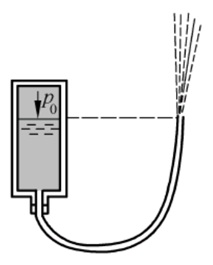
\includegraphics[width=\textwidth]{asset/ch2/T20.png}
    \end{minipage}
\end{example}